\section{Metathesis and identity}\label{sec:MetIde}

\begin{figure}[h]
	\caption{Self-identified varieties of Meto}\label{fig:SelIdeVarUabMeto-2}
	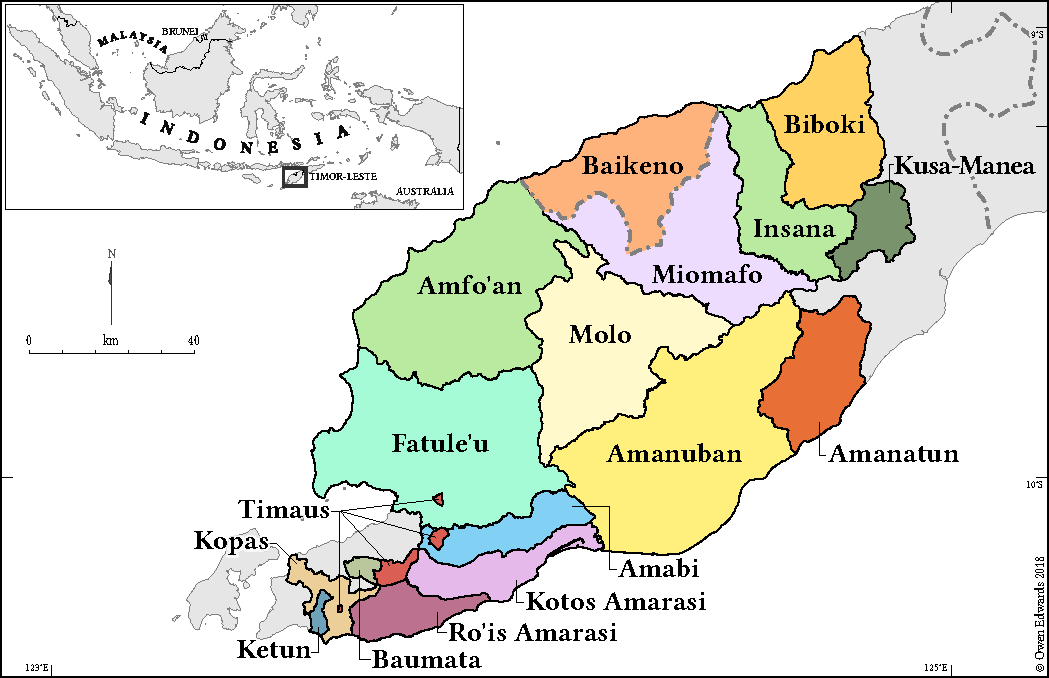
\includegraphics[width=\columnwidth]{Metos-LinLib.pdf}
\end{figure}

It is well known that language is frequently employed
as a marker of identity \citep{mi82,ed09,figa10}.
This is also the case in western Timor in which the four
main ethnic identities are delineated according to language:
Rote, Helong, Tetun, and the Atoni, who speak Meto.\footnote{
		Meto speakers refer to themselves in full as \ve{atoin paah metoʔ}
		or \ve{atoni paah metoʔ} `people of the dry land' (\citealt[i]{cu62}; \citealt[1]{scno71}).
		The term Atoni is from \ve{atoniʔ} in Amarasi
		or \ve{atoni} in other Meto varieties and means `man, person'.}

Within each of these groups, further identities also exist.
While the Atoni (Meto speakers) self-identify as
a single cultural and linguistic group,
they also acknowledge internal cultural and linguistic differences between groups.
The labels used for the prescriptively defined different groups,
as given in \frf{fig:SelIdeVarUabMeto-2},
correspond almost exactly to the historic kingdoms of the region.

One kind of cultural difference found between groups is different weaving traditions.
An example of Amarasi cloth, Amfo{\Q}an cloth, and Fatule{\Q}u cloth
is given in \frf{fig:ThrTypMetClo} below.
Further differences in weaving are also found between individual hamlets.
Thus, the use of blue lines between the geometric maroon patterns
in \frf{fig:AmaClo} is distinctive of Koro{\Q}oto hamlet
while the hamlet of Ponain, for instance, mainly uses yellow lines.

\begin{figure}[h]
  \begin{subfigure}[b]{0.32\textwidth}
		\frame{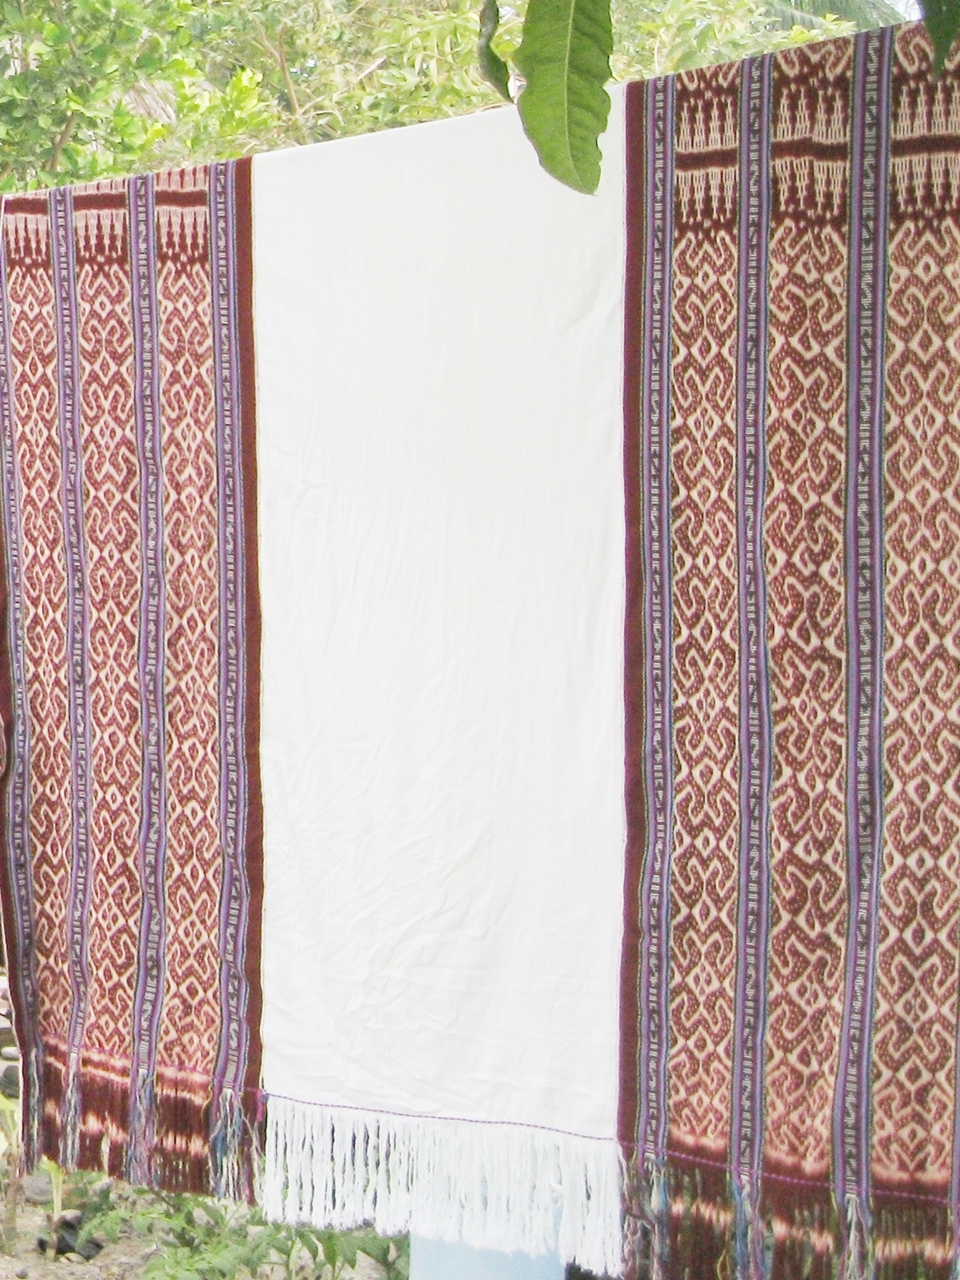
\includegraphics[width=\linewidth]{AmarasiCloth.jpg}}
		\caption{Amarasi cloth}\label{fig:AmaClo}
  \end{subfigure}
  \begin{subfigure}[b]{0.32\textwidth}
		\frame{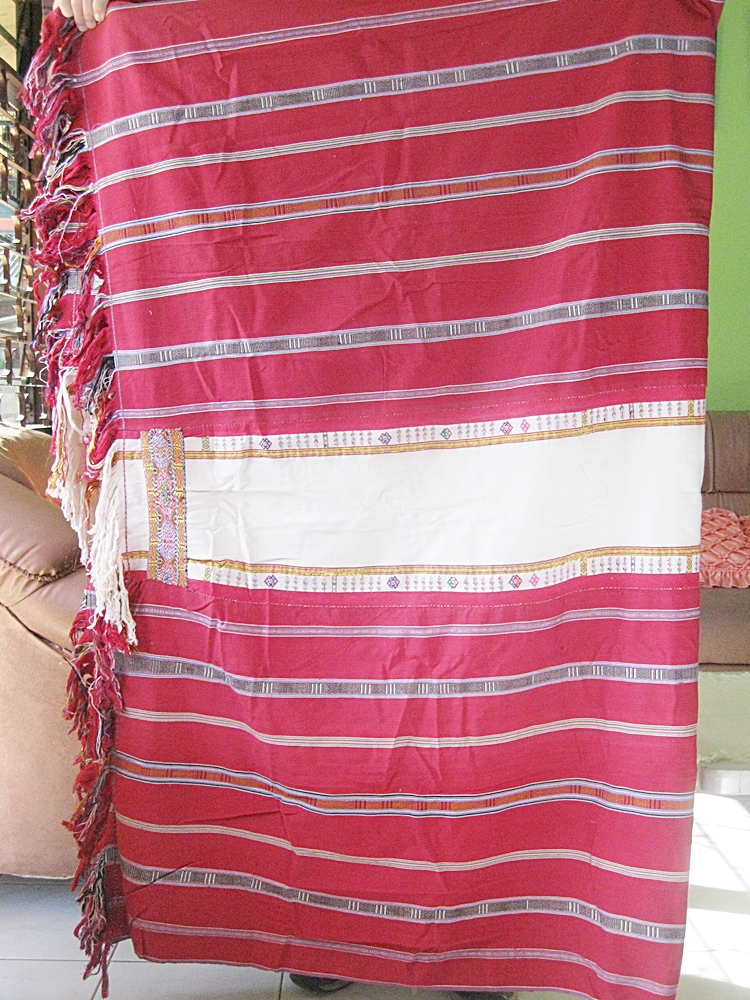
\includegraphics[width=\linewidth]{AmfoanCloth.jpg}}
		\caption{Amfo{\Q}an cloth}\label{fig:AmfClot}
  \end{subfigure}
  \begin{subfigure}[b]{0.32\textwidth}
		\frame{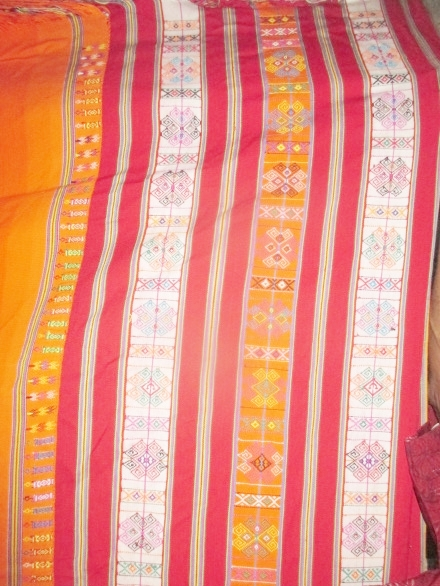
\includegraphics[width=\linewidth]{FatulequCloth.jpg}}
		\caption{Fatule{\Q}u cloth}\label{fig:FatClot}
  \end{subfigure}
	\caption{Three types of Meto cloth}\label{fig:ThrTypMetClo}
\end{figure}

Another example of enacted identity can be found in the 
different methods employed to count corn,
the traditional crop of western Timor.
As reported by \cite{grba11}, Kotos Amarasi counts
corn in units of \ve{rean}, with one \ve{rean} being 400 cobs of corn.
In the Tais Nonof variety of Amarasi,
corn is counted by the \ve{nifu} (thousand).
In some other regions corn is counted by \it{kuda} (Indonesian for `horse')
with one \it{kuda} consisting of 80 cobs of corn.

Such differences are salient to the Atoni.
When collecting data on Fatule{\Q}u I was accompanied
by my main Amarasi consultant, Heronimus Bani (Roni).
After I had collected a word-list,
Roni asked about cloth design in Fatule{\Q}u;
what the different parts of the pattern were called,
and what these patterns symbolised, in fact
figure \frf{fig:FatClot} was taken by Roni.
He also asked how corn was counted in Fatule{\Q}u
and volunteered that in Amarasi corn was counted by \ve{rean}.

The Atoni agree that they speak a single language: Meto.
However, they also acknowledge that there are differences in how people speak
in different places, differences which can often accumulate to such an
extent that they seriously hinder communication.

In my experience, Atoni from different regions
often talk in a mixture of Meto and Indonesian/Kupang Malay.
The use of Meto enables expression of their shared identity and
the use of Indonesian/Kupang Malay enables effective communication.
One or more speakers will also usually adapt their speech to
perceived norms of their interlocutors.

The Atoni are aware to varying degrees of salient differences between different varieties of Meto.
It is fairly common knowledge, for instance, that Amarasi has /r/ while
other varieties have /l/.\footnote{
		The situation is, in fact, more complex.
		Amabi and Kusa-Manea also have /r/ instead of /l/.
		Timaus has both /l/ and /r/
		(the latter of which has developed from *\j).
		These additional complexities do not enter into the
		popular discourse about differences.}
Similarly, on a more local scale speakers of Kotos Amarasi and Ro{\Q}is Amarasi
are aware of some differences between one another's speech,
and when asked, my Kotos consultants would gleefully try to imitate Ro{\Q}is speech.

One obvious kind of linguistic difference between
different varieties of Meto is lexical.
A selection of lexemes in several varieties of Meto
and other languages of western Timor is given in \trf{tab:LexDifUabMetVar}.
Although the difference between Meto other languages
is greater than that between individual varieties of Meto,
the internal diversity of Meto is not insignificant.

\begin{table}[h]
	\caption{Lexical differences between languages of western Timor}\label{tab:LexDifUabMetVar}
	\centering
	\begin{threeparttable}
	\stl{0.3em}\begin{tabular}{rllllll} \lsptoprule
									& `earth'					& `thorn'				& `mouse'			& `red'\su{†}		&	`big'					& `dream' 			\\ \midrule
			Amarasi			&	\ve{afu}				& \ve{aikaʔ}		& \ve{knafo}	& \ve{meʔe}			&	\ve{koʔu}			& \ve{na-mnei}	\\
			Amanuban		&	\ve{nain}				& \ve{sakunat}	& \ve{nafo}		& \ve{meeʔ}			&	\ve{ʔnaek}		& \ve{na-naeʔ}	\\
			Amanatun		&	\ve{nain}				& \ve{kasunat}	& \ve{nafo}		& \ve{meeʔ}			&	\ve{ʔnaek}		& \ve{na-naeʔ}	\\
			Fatule{\Q}u	&	\ve{afu}				& \ve{}					& \ve{ifo}		& \ve{mtasaʔ}		&	\ve{ʔnaek}		& \ve{n-unmaeʔ}	\\
			Molo				&	\ve{na\j an}		& \ve{katilaʔ}	& \ve{ifo}		& \ve{mtasaʔ}		&	\ve{ʔnaek}		& \ve{n-ʔunmaeʔ}\\
			Amfo{\Q}an	&	\ve{nai\j an}		& \ve{kalilaʔ}	& \ve{ifog}		& \ve{mtasaʔ}		&	\ve{ʔnaek}		& \ve{na-smaan}	\\
			Baikeno			&	\ve{nai\j aan}	& \ve{kalilaʔ}	& \ve{bifo}		& \ve{meeʔ}			&	\ve{ʔnaek}		& \ve{na-mnei}	\\
			Timaus			&	\ve{afi\j}			& \ve{katilaʔ}	& \ve{ifugw}	& \ve{meeʔ}			&	\ve{ʔnaek}		& \ve{n-mai}		\\
			Kopas				&	\ve{afu}				& \ve{katilaʔ}	& \ve{ifo}		& \ve{meeʔ}			&	\ve{ʔnaek}		& \ve{na-mnai}	\\
			Kusa-Manea	&	\ve{nian}				& \ve{tanaʔ}		& \ve{nafo}		& \ve{nuti}			&	\ve{binaiʔ}		& \ve{na-mnei}	\\ \hline
			Helong			&	\it{dale}				& \it{duliʔ}		& \it{blaho}	& \it{mea}			&	\it{tene}			& \it{natloa}		\\
			Lole (Rote)	&	\it{dae}				& \it{dilak}		& \it{lafo}		& \it{mbilas}		&	\it{inahuu-k}	& \it{meʔi}			\\
			Dela (Rote)	&	\it{rae}				& \it{maŋgouʔ}	& \it{lafo}		& \it{mbilas}		&	\it{ine-ʔ}		& \it{na-lamein}\\
			Tetun				&	\it{rai}				& \it{ktarak}		& \it{laho}		& \it{mean}			&	\it{boo}			& \it{meʔi}			\\ \lspbottomrule
		\end{tabular}
			\begin{tablenotes}
				\item[†] In Amarasi \ve{mtasaʔ} means `ripe' and \ve{meʔe mtasaʔ} `maroon'.
			%%	\item[‡]
			%%	\item[§]
			%%	\item[‖] 
			%%	\item[¶] 
			\end{tablenotes}
	\end{threeparttable}
\end{table}

\subsection{Realisation of U-forms and M-forms}
Another marker of linguistic identity among the Atoni is metathesis: different ways of realising
U-forms and M-forms, different environments in which these forms are used
and different functions of these forms.
Some differences in the realisation of U-forms and M-forms
between eight different varieties of Meto
are given in \trf{tab:VarUfoMfo},
with identical forms indicated by identical colours.

\begin{table}[h]
	\caption[Variation in U-forms and M-forms]
					{Variation in U-forms and M-forms\su{†}}\label{tab:VarUfoMfo}
	\centering\stl{0.2em}
		\begin{threeparttable}
			\begin{tabular}{rllllllllll}\lsptoprule
	&	\mc{2}{l}{`three'} 					&	\mc{2}{l}{`dog'} 					&	\mc{2}{l}{`wood, tree'} 					&	\mc{2}{l}{`fire'} 					&	\mc{2}{l}{`day'} 					\\	\midrule
	&	\tsc{u}		&	\tsc{m}		&	\tsc{u}		&	\tsc{m}		&	\tsc{u}		&	\tsc{m}		&	\tsc{u}		&	\tsc{m}		&	\tsc{u}		&	{\Mvv}		\\	
Kotos\sub{\tsc{k}}	&	\it{tenu}	{\cellcolor{blue!40}}	&	\it{teun}	{\cellcolor{blue!40}}	&	\it{asu}	{\cellcolor{blue!40}}	&	\it{aus}	{\cellcolor{blue!40}}	&	\it{hau}	{\cellcolor{blue!40}}	&	\it{hau}	{\cellcolor{blue!40}}	&	\it{ai}	{\cellcolor{blue!40}}	&	\it{ai}	{\cellcolor{blue!40}}	&	\it{neno}	{\cellcolor{blue!40}}	&	\it{neeŋgw=}	{\cellcolor{blue!40}}	\\	
Kotos\sub{\tsc{f}}	&	\it{tenu}	{\cellcolor{blue!40}}	&	\it{teun}	{\cellcolor{blue!40}}	&	\it{asu}	{\cellcolor{blue!40}}	&	\it{aus}	{\cellcolor{blue!40}}	&	\it{hau}	{\cellcolor{blue!40}}	&	\it{hau}	{\cellcolor{blue!40}}	&	\it{ai}	{\cellcolor{blue!40}}	&	\it{ai}	{\cellcolor{blue!40}}	&	\it{neno}	{\cellcolor{blue!40}}	&	\it{neoŋg=}	{\cellcolor{green!50}}	\\	
Ro{\Q}is\sub{\tsc{s}}	&	\it{tenu}	{\cellcolor{blue!40}}	&	\it{teun}	{\cellcolor{blue!40}}	&	\it{asu}	{\cellcolor{blue!40}}	&	\it{aus}	{\cellcolor{blue!40}}	&	\it{hau}	{\cellcolor{blue!40}}	&	\it{hau}	{\cellcolor{blue!40}}	&	\it{ai}	{\cellcolor{blue!40}}	&	\it{ai}	{\cellcolor{blue!40}}	&	\it{neno}	{\cellcolor{blue!40}}	&	\it{neenb=}	{\cellcolor{yellow!75}}	\\	
Amanub.	&	\it{tenu}	{\cellcolor{blue!40}}	&	\it{teun}	{\cellcolor{blue!40}}	&	\it{asu}	{\cellcolor{blue!40}}	&	\it{aus}	{\cellcolor{blue!40}}	&	\it{hau}	{\cellcolor{blue!40}}	&	\it{hau}	{\cellcolor{blue!40}}	&	\it{ai}	{\cellcolor{blue!40}}	&	\it{ai}	{\cellcolor{blue!40}}	&	\it{neno}	{\cellcolor{blue!40}}	&	\it{neen=}	{\cellcolor{orange!85}}	\\	
%Ketun	&	\it{tenu}	{\cellcolor{blue!40}}	&	\it{teun}	{\cellcolor{blue!40}}	&	\it{asaw}	{\cellcolor{green!50}}	&	\it{aus}	{\cellcolor{blue!40}}	&	\it{hau}	{\cellcolor{blue!40}}	&	\it{hau}	{\cellcolor{blue!40}}	&	\it{ai}	{\cellcolor{blue!40}}	&	\it{ai}	{\cellcolor{blue!40}}	&	\it{nenao̯}	{\cellcolor{green!50}}	&			\\	
Kualiin	&	\it{tenu}	{\cellcolor{blue!40}}	&	\it{teun}	{\cellcolor{blue!40}}	&	\it{asaw}	{\cellcolor{green!50}}	&	\it{aus}	{\cellcolor{blue!40}}	&	\it{hau}	{\cellcolor{blue!40}}	&	\it{hau}	{\cellcolor{blue!40}}	&	\it{ai}	{\cellcolor{blue!40}}	&	\it{ai}	{\cellcolor{blue!40}}	&	\it{nenao̯}	{\cellcolor{green!50}}	&	\it{neen=}	{\cellcolor{orange!85}}	\\	
Baikeno	&	\it{tenu}	{\cellcolor{blue!40}}	&	\it{teen}	{\cellcolor{green!50}}	&	\it{asu}	{\cellcolor{blue!40}}	&	\it{aos}	{\cellcolor{green!50}}	&	\it{haub}	{\cellcolor{green!50}}	&	\it{hau}	{\cellcolor{blue!40}}	&	\it{ai\j}	{\cellcolor{green!50}}	&	\it{ai}	{\cellcolor{blue!40}}	&	\it{neno}	{\cellcolor{blue!40}}	&	\it{neemb=}	{\cellcolor{red!70}}	\\	
Amfo{\Q}an	&	\it{tenu}	{\cellcolor{blue!40}}	&	\it{teen}	{\cellcolor{green!50}}	&	\it{asug}	{\cellcolor{yellow!75}}	&	\it{asu}	{\cellcolor{yellow!75}}	&	\it{haug}	{\cellcolor{yellow!75}}	&	\it{hau}	{\cellcolor{blue!40}}	&	\it{ai\j}	{\cellcolor{green!50}}	&	\it{ai}	{\cellcolor{blue!40}}	&	\it{nenog}	{\cellcolor{yellow!75}}	&	\it{neeŋgw=}	{\cellcolor{blue!40}}	\\	
Timaus	&	\it{tenu}	{\cellcolor{blue!40}}	&	\it{teenw}	{\cellcolor{yellow!75}}	&	\it{asi\j}	{\cellcolor{orange!85}}	&	\it{asu}	{\cellcolor{yellow!75}}	&	\it{haa\j}	{\cellcolor{orange!85}}	&	\it{hau}	{\cellcolor{blue!40}}	&	\it{aar}	{\cellcolor{yellow!75}}	&	\it{ai}	{\cellcolor{blue!40}}	&	\it{nenugw}	{\cellcolor{orange!85}}	&	\it{neeŋgw=}	{\cellcolor{blue!40}}	\\	
Fatule{\Q}u	&	\it{tenu}	{\cellcolor{blue!40}}	&	\it{teenw}	{\cellcolor{yellow!75}}	&	\it{asu}	{\cellcolor{blue!40}}	&	\it{aus}	{\cellcolor{blue!40}}	&	\it{haub}	{\cellcolor{green!50}}	&	\it{hau}	{\cellcolor{blue!40}}	&	\it{aa\j}	{\cellcolor{orange!85}}	&	\it{ai}	{\cellcolor{blue!40}}	&	\it{neno}	{\cellcolor{blue!40}}	&	\it{neenb=}	{\cellcolor{yellow!75}}	\\	
Kopas\sub{\tsc{t}}	&	\it{tenu}	{\cellcolor{blue!40}}	&	\it{teun}	{\cellcolor{blue!40}}	&	\it{asu}	{\cellcolor{blue!40}}	&	\it{aus}	{\cellcolor{blue!40}}	&	\it{haag}	{\cellcolor{red!70}}	&	\it{hau}	{\cellcolor{blue!40}}	&	\it{aa\j}	{\cellcolor{orange!85}}	&	\it{ai}	{\cellcolor{blue!40}}	&	\it{neno}	{\cellcolor{blue!40}}	&	\it{neon=}	{\cellcolor{purple!75}}	\\	
Kopas\sub{\tsc{u}}	&	\it{tenu}	{\cellcolor{blue!40}}	&	\it{teenw}	{\cellcolor{yellow!75}}	&	\it{asu}	{\cellcolor{blue!40}}	&	\it{aus}	{\cellcolor{blue!40}}	&	\it{haagw}	{\cellcolor{purple!75}}	&	\it{hau}	{\cellcolor{blue!40}}	&	\it{aa\j}	{\cellcolor{orange!85}}	&	\it{ai}	{\cellcolor{blue!40}}	&	\it{neno}	{\cellcolor{blue!40}}	&			\\	
			\lspbottomrule
			\end{tabular}
				\begin{tablenotes}
					\item [\su{†}]	Kotos\sub{\tsc{k}} = Kotos Amarasi from Koro{\Q}oto hamlet,
													Kotos\sub{\tsc{f}} = Kotos Amarasi from Fo{\Q}asa{\Q} hamlet,
													Ro{\Q}is\sub{\tsc{s}} = Ro{\Q}is Amarasi from Suit hamlet,
												%	Amarasi\sub{\tsc{f}} = Kotos Amarasi from Fo{\Q}asa{\Q} hamlet,
													Amanub. = Amanuban from Niki-niki,
												%	Baikeno = 
													Kualiin = Amanuban from Kualin village,
													Amfo{\Q}an = Naitbelak Amfo{\Q}an from Ta{\Q}en hamlet,
													Fatule{\Q}u = Bineon-Koa{\Q} hamlet,
													Kopas\sub{\tsc{t}} = Tuale{\Q}u hamlet,
													Kopas\sub{\tsc{u}} = Usapisonba{\Q}i hamlet,
				\end{tablenotes}
		\end{threeparttable}
\end{table}

\trf{tab:VarUfoMfo} shows that there is an extensive array
of realisations for U-forms and M-forms.
The four different process which occur are: metathesis,
consonant insertion, diphthongisation, and vowel shift or assimilation.
Different combinations of these processes not only occur in different Meto varieties,
but two particular varieties of Meto do not necessarily treat all words
of the same phonotactic shape in the same way.

Nouns undergo metathesis in all (known) varieties before vowel initial enclitics,
but with or without insertion of different consonants
(which occurs with or without assimilation of final /n/).
A number of varieties mark U-forms ending in a vowel sequence
by consonant insertion, though in different varieties different consonants are inserted
and are accompanied by different degrees of vowel assimilation.
Words which end in CV{\#} can have basic M-forms
marked by metathesis (with presence or lack of various kinds of vowel assimilation)
or by lack of consonant insertion, with some Meto varieties
also showing variation between different word classes.

In the context of other linguistic alternations and markers of identity,
such differences in the realisation of U-forms and M-forms
are an additional strategy for marking linguistic identity.
They are also perceived this way by both insiders and outsiders.

In her analysis of consonant insertion in Nai{\Q}bais Amfo{\Q}an
\cite{cu18} reports this process is seen by
speakers as a marker of identity.
Thus, \citeauthor{cu18}'s main consultant told her when she began her work:
{``Here in Amfo{\Q}an we add consonants at the end of sentences.
That's how you know someone is from Amfo{\Q}an.''}
Similarly, this process is viewed by outsiders as distinctive.
When I collected Amfo{\Q}an data I was accompanied
by speakers of Amanuban from So{\Q}e.
On the way up to Amfo{\Q}an, my friends reported
that ``all the words there end in <g>'',
referring to the process of consonant insertion used to form the U-forms
of nouns which end in /o/ and /u/ (\srf{sec:EmpCSloConIns}).

Similarly, Amarasi speakers from Koro{\Q}oto
hamlet know that speakers from Fo{\Q}asa{\Q} hamlet have different M-forms before enclitics
(e.g. Koro{\Q}oto \ve{nee{\ng}gw=ee}, Fo{\Q}asa{\Q} \ve{neo{\ng}g=ee} `the sky, day').
Likewise, when collecting data on Fatule{\Q}u, Kopas and Timaus while accompanied
by Roni (my main Amarasi consultant), the different patterns
of metathesis and consonant insertion in these
Meto varieties were very salient to him.

Furthermore, differences in the realisation of U-forms and M-forms
are quite difficult for speakers of different varieties of Meto to copy.
In discussions with Roni after collecting Timaus data, he was generally unable to reproduce
the kinds of consonant insertion seen there, despite the correspondences
between Amarasi and Timaus being regular.

Similarly, I have overheard speakers of Amanuban
attempt, but fail, to correctly copy patterns of metathesis in Amarasi.
While Amanuban speakers know there are differences in
vocabulary and metathesis between their speech and Amarasi,
they are not necessarily able to combine the two together correctly.
This is in contrast with other some other differences,
such as the use of /r/ in Amarasi where Amanuban has /l/.

Compare examples \qf{ex:AmanubanMet} and \qf{ex:AmarasiMet} below,
which shows the same way of saying a number of phrases in Amanuban and Amarasi.
In both varieties verbs before the inceptive enclitic \ve{=een} undergo consonant insertion,
metathesis and vowel assimilation, but with different consonants inserted.
Where Amarasi inserts /ɡw/, Amanuban inserts /w/
and where Amarasi inserts /\j/, Amanuban inserts a palatal glide /j/.

\begin{multicols}{2}
	\begin{exe}
		\ex{Amanuban:}\label{ex:AmanubanMet}
			\begin{xlist}
				\ex{\glll	hai m-faan\tbr{j}=een.\\
									hai m-fani=ena\\
									{\hai} \m-back{\Mv}={\een}\\
						\glt	`We'll head back now.'}
				\ex{\glll	hai m-naa\tbr{w}=een.\\
									hai m-nao=ena\\
									{\hai} \m-go{\Mv}={\een}\\
						\glt	`We'll get going now.'}
				\ex{\glll	hai m-\tbr{fiinj}=een.\\
									hai m-fini=ena\\
									{\hai} \m-pass{\Mv}={\een}\\
						\glt	`We'll keep going now.'}
			\end{xlist}
		\ex{Amarasi:}\label{ex:AmarasiMet}
			\begin{xlist}
				\ex{\glll	hai m-faan\tbr{\j}=een.\\
									hai m-fani=ena\\
									{\hai} \m-back{\Mv}={\een}\\
						\glt	`We'll head back now.'}
				\ex{\glll	hai m-naa\tbr{gw}=een.\\
									hai m-nao=ena\\
									{\hai} \m-go{\Mv}={\een}\\
						\glt	`We'll get going now.'}
				\ex{\glll	hai m-\tbr{koo\ng gw}=een.\\
									hai m-kono=ena\\
									{\hai} \m-pass{\Mv}={\een}\\
						\glt	`We'll keep going now.'}
			\end{xlist}
	\end{exe}
\end{multicols}

In addition to the differences in consonant insertion,
there are also differences in vocabulary:
Amarasi has \ve{{\rt}kono} `pass' and Amanuban has \ve{{\rt}fini} `pass'.
While Amanuban speakers are aware of such differences,
they are not necessarily able to combine the two together.
The top line of example \qf{ex:AmarasiError} below was said
by one of my Amanuban friends when trying to adapt
their speech to Amarasi.

\begin{exe}\let\eachwordtwo=\ve\let\eachwordthree=\ve
	\ex{\glll	\textnormal{\tcb{incorrect Amarasi:}} 			hai m-koom\j=een.		\,\,\textnormal{\tcb{{\la} hai m-komi=een}} \\
						\textnormal{\tcb{\hp{in}correct Amarasi:}}	hai m-koo{\ng}gw=een.	\,\,\textnormal{\tcb{{\la} hai m-kono=een}} \\
						\textnormal{\tcb{\hp{in}correct Amanuban:}}	hai m-fiinj=een.			\,\,\textnormal{\tcb{{\la} hai m-fini=een}}\\
				\glt		\lh{incorrect Amanuban:} `We'll keep going now.' \txrf{observation}}\label{ex:AmarasiError}
\end{exe}

In this example, the Amanuban speaker has had some success
in selecting the correct verb, though has selected the wrong medial nasal with /m/ instead of /n/.\footnote{
		The selection of the incorrect nasal /m/ rather than correct
		/n/ probably came about partly in order to differentiate
		this form from \ve{{\rt}koni} `copulate'.}
They have also correctly identified a rule along the lines of
``Amarasi inserts /\j/ where we insert /j/''.
Because of this they have inserted /\j/ for this sentence.
However, the difference in the quality of the final vowels of
Amarasi \ve{{\rt}kono} `pass' and Amanuban \ve{{\rt}fini} `pass'
means that application of this rule yields an incorrect result in this instance.

\subsection{Environments for U-forms and M-forms}
The realisation of the U-form and M-form of words
is one dimension across which speakers of Meto can mark identity.
Another dimension is the environments in which metathesis occurs.
For instance, in Kotos Amarasi metathesis is blocked before words
which begin with a consonant cluster (\srf{sec:CCIniMod}),
while in Ro{\Q}is Amarasi metathesis freely occurs
before such words (\srf{sec:RoqAnaCCIniMod}).
This yields pairs such as Kotos \ve{u\tbr{mi} kbubuʔ} and Ro{\Q}is \ve{u\tbr{im} kbubuʔ} `round house',
or Kotos \ve{kru\tbr{ru} tnana-f} Ro{\Q}is \ve{kru\tbr{ur} tnana-f} `middle finger'.
More examples are given in \trf{tab:RoqMetConClu} on \prf{tab:RoqMetConClu}.

Similarly, consonant final verbs do not undergo
metathesis in Kotos Amarasi (\srf{sec:ConFinVer}),
while in Ro{\Q}is Amarasi verbs with a final /n/ are eligible
to undergo metathesis (\srf{sec:MforFinConClu}).
Two examples of Ro{\Q}is phrases with metathesis
resulting in a final consonant cluster are given in \qf{ex:08/10/14, p.113 ch:ConCon}
and \qf{ex:09/10/14, p.114 ch:ConCon} below along with their Kotos equivalents.

\begin{multicols}{2}
	\begin{exe}\let\eachwordtwo=\ve
		\ex{\glll	\textnormal{\tcb{Ro{\Q}is:}} siin na-sa\tbr{ap}=\tbr{n}.\\
							\textnormal{\tcb{Kotos:}} siin na-sa\tbr{pa}=\tbr{n}.\\
							{} {\siin} {\na}-kick={\einV}\\
				\glt	\lh{Kotos: }`They're playing soccer.'}\label{ex:08/10/14, p.113 ch:ConCon}
							%\txrf{observation 08/10/14, p.113}}\label{ex:08/10/14, p.113 ch:ConCon}
		\ex{\glll	\textnormal{\tcb{Ro{\Q}is:}} raump=ein n-ma\tbr{et}=\tbr{n}.\\
							\textnormal{\tcb{Kotos:}} paku=n n-ma\tbr{te}=\tbr{n}.\\
							{} light={\ein} {\n}-die={\einV}\\
				\glt	\lh{Kotos: }`The lights have died.'}\label{ex:09/10/14, p.114 ch:ConCon}
							%\txrf{observation 09/10/14, p.114}}\label{ex:09/10/14, p.114 ch:ConCon}
	\end{exe}
\end{multicols}

Another dimension across which differences in metathesis
can be marked is in the functions of U-forms and M-forms.
In this book I have described and analysed the functions of U-forms and M-forms
only in Kotos Amarasi (as spoken in Koro{\Q}oto hamlet).
Although the full details remain to be investigated,
data from other varieties of Meto shows that metathesis
behaves differently in different varieties.

Thus, for instance, in Amfo{\Q}an \citep{cu18}
and Timaus (own fieldnotes) verbs take the U-form
much more often than they do in Kotos Amarasi.
This is clearly exemplified in \qf{ex:Mark 1:2}--\qf{ex:Mark 16:7}
below with a selection of parallel passages from the gospel
of Mark in Amarasi and Amfo{\Q}an \citep{UBB18}.
The Amfo{\Q}an version is given below the Amarasi.
Verbs which are metathesised in Amarasi but
unmetathesised in Amfo{\Q}an are indicated.

\begin{exe}\let\eachwordtwo=\ve
	\ex{\glll	na-hu\tbr{un} na-ʔko naiʔ Yesus n-a\tbr{it}  iin mepu,\\
						na-hu\tbr{nu} na-ʔko nai  Yesus n-a\tbr{iti} iin mepug,\\
						\na-first \na-{\qko} {\naiq} Jesus \n-pick.up {\iin} work\\
			\glt	`Before Jesus began his work,' \txrf{Mark 1:2a}}\label{ex:Mark 1:2}
	\ex{\glll	n-ok ranan mee henatiʔ paah naan \hp{na-}bisa {\a}n-ha\tbr{ek} na-ba\tbr{ar}?\\
						na-tuin lalan mee henatiʔ paah naan na-beʔi a|n-ha\tbr{ke} na-ba\tbr{la}?\\
						3-with way what {\he} country {\naan} 3-able \a\n-stand \na-constant\\
			\glt	`In what way will that country be able to endure?'\txrf{Mark 3:24}}\label{ex:Mark 3:24}
	%\ex{\glll	a|n-bi oors =ees, siin n-e\tbr{ik} siin aanh =ein nema=n n-eu naiʔ Yesus\\
						%a|n-bi tabug meseʔ, sini n-e\tbr{ki} siin anah =siin nema=n n-oi nai  Yesus\\
						%\n-{\ek} time one {\siin} \n-bring {\siin} child ={\ein} come={\einV} \n-{\eu} {\naiq} Jesus\\
			%\glt	`One time, they brought their children to Jesus'\txrf{Mark 10:13}}\label{ex:Mark 10:13}
	\ex{\glll	ma oras maans =ii {\a}n-ma\tbr{eb} on nana =te\\
						ma tabug manas {} a|n-ma\tbr{be} on nane\\
						and time sun ={\ii} \a\n-afternoon like {\naan} ={\te}\\
			\glt	`And when the sun was about to go down,'\txrf{Mark 11:19}}\label{ex:Mark 11:19}
	\ex{\glll	onaim hii {\a}m-fa\tbr{in} nai rab{\tl}raab! \\
						{ees on naan} hii a|m-fa\tbr{ni} nai lab{\tl}laab!\\
						and.so {\hii} \a\m-return already {\prd}quick\\
			\glt	`So return quickly!'\txrf{Mark 16:7}}\label{ex:Mark 16:7}
%	\ex{\glll	\\
%						\\
%						\\
%			\glt	`'\txrf{}}\label{ex:}
\end{exe}

The Amfo{\Q}an gospel of Mark has been translated
by native speakers from the Amarasi version.
This means that the differences in metathesis seen
in \qf{ex:Mark 1:2}--\qf{ex:Mark 16:7} above
reflect deliberate decisions by Amfo{\Q}an speakers
to unmetathesise certain verbs to yield a more natural translation.

While the exact function of metathesis in Amfo{\Q}an
discourse remains to be fully worked out,
it is clear that the analysis I proposed for Amarasi
in Chapter \ref{ch:DisMet} cannot be straightforwardly
extended to cover the Amfo{\Q}an data.

\begin{table}[h]
	\centering\caption{Bird names in Timaus}\label{tab:BirNamTim}
	\begin{tabular}{rll}\lsptoprule
		Head			&	Modifier			&	gloss	\\	\midrule
		\ve{kolo}	&	\ve{anal}			&	`sparrow'	\\	
		\ve{kolo}	&	\ve{fumaki\j}	&	`orange-banded thrush'	\\	
		\ve{kolo}	&	\ve{kael}			&	`yellow-crested cockatoo'	\\	
		\ve{kolo}	&	\ve{kefar}		&	`pigeon'	\\	
		\ve{kolo}	&	\ve{kuis}			&	`thrush'	\\	
		\ve{kolo}	&	\ve{luan}			&	`wild pigeon'	\\	
		\ve{kolo}	&	\ve{kaaʔ}			&	`crow'	\\	\hline
		\ve{kool}	&	\ve{kaaʔ}			&	`crow'	\\	
		\ve{kool}	&	\ve{kitaʔ}		&	`great-billed parrot'	\\	
		\ve{kool}	&	\ve{kuki\j}		&	`collared dove'	\\	
		\ve{kool}	&	\ve{otos}			&	`barred dove'	\\	
		\lspbottomrule
	\end{tabular}
\end{table}

Regarding metathesis in the syntax, my Timaus
data shows that certain noun phrases occur
with a metathesised head while others do not.
In my Timaus data I have ten names of different
kinds of birds composed of the noun \ve{kolo} `bird'
(phrase final \ve{kolugw}) followed by a nominal modifier.
Of these, the head is metathesised in six,
unmetathesised in four, and one shows variation.
These Timaus bird names are given in \trf{tab:BirNamTim}.
Whatever the basis for this variation in Timaus,
it is clearly different from Amarasi in which head
nouns obligatorily occur metathesised when
followed by an attributive modifier.

Similarly, in Insana data given by \cite{scno71},
certain noun phrases have an unmetathesised head
while others have a metathesised head.
Examples of phrases with a metathesised head include
\ve{lais metoʔ} `traditional matters' (Amarasi \ve{rais metoʔ}),
and \ve{neon tees} `sunset' (Amarasi \ve{neon tees}).
Examples of phrases with an unmetathesised head include \ve{mone feʔu} `son-in-law,
\emph{lit.} new male' (Amarasi \ve{moen feʔu}) and
\ve{tasi mone} `southern sea, \emph{lit.} male sea' (Amarasi \ve{tais mone}).
Again, this reflects a different use of metathesis in the syntax
between Insana and Amarasi.

Metathesis is a marker of identity within the Atoni ethno-linguistic group.
The presence of metathesis in this language cluster
sets it apart from other local groups, such as Tetun and the Rote languages
-- though not from Helong (\srf{sec:Hel}) --
and the differences between the forms, functions and environments
of metathesis between different varieties of Meto
vary and serve to mark sub-identities among the Atoni.